%*******************************************************
% Abstract
%*******************************************************
%\renewcommand{\abstractname}{Abstract}

\begingroup
\let\clearpage\relax
\let\cleardoublepage\relax
\let\cleardoublepage\relax

\begin{otherlanguage}{english}
\pdfbookmark[1]{Abstract}{Abstract}
\chapter*{Extended Abstract}

Nowadays, to proof someone we know a certain secret, we shall use a transmission channel where nobody could spy on us, and then we send the secret directly to our listener. In the scope of cryptography, we would cipher the secret with a key, in a symmetric or asymmetric scheme, such that only those who know the deciphering key can actually read our encrypted secret. This is the foundation of the Internet's security. We cipher our password in a way only the mail server can read it, so it deciphers the password and if it matches the one stored in its side, the server lets you log in and access to your account, without any eavesdropper stealing our password in between. The problem here is that the password is only secured during the transmission, two entities know the secret and therefore we have two possible points of attack where a malicious entity would not need to break de ciphering scheme used in the transmission channel.

There exists a special area in cryptology in charge of studying this issue, proving someone we know something, but that from the proof performed, no other information is obtained, except that the proof itself is correct. These methods are known as Zero-Knowledge Proofs, because they leak no extra knowledge from performing them.
We chose to study these techniques due to the Computer Science degree thesis, \textit{Integration of Idemix in IoT environments}, where Idemix is a cryptographic protocol based on zero-knowledge proofs. When we started the study of said thesis, we noticed the amount of mathematical results related, for this reason, we were interested in studying it deeply and formally, and considered it for this Mathematics degree thesis.

To illustrate how zero-knowledge proofs work, in 1990 Guillou, Quisquater and Berson published in \textit{How to Explain Zero-Knowledge Protocols to Your Children} \citep{ZKPcave:story} a story about how Ali Baba proved he was able to open the door of the cave, without revealing anyone the magic words. Due to it being a 4 pages long story, here we present a brief version which highlights the basic properties of these methods:

\hfil

\begin{quote}
	Imagine a cave, where the path forks in two passages, and at the end of each one, they join again, with the shape of a ring. In the point the paths meet, there is a magic door, that only opens when someones pronounces the magic work.
	
	\textbf{P}eggy knows the secret word and wants to \textbf{p}rove it to her friend, \textbf{V}ictor, but without revealing it.
	Peggy and Victor meet at the entrance of the cave, then Victor awaits while Peggy goes inside the cave, taking one of the passages, that we will name A and B. Victor can't see which way Peggy went. 
	
	When Peggy arrives at the door, \textbf{V}ictor enters the cave, and when he arrive to the fork, stops and yells which path, A or B, he wants Peggy to come back, to \textbf{v}erify she knows how to open the door.
		
	If Peggy actually knows the secret, she always can take the requested path, opening the magic door if needed.
	But if Peggy doesn't know the magic word, she had a chance of $50\%$ to guess correctly what passage Victor was going to ask. That means she had a chance to fool Victor.
	
	Victor then asks to repeat the experiment. With $20$ repetitions, the chances Peggy fools Victor in all of them is only  $2^{-20}$, practically negligible, of guessing every time and therefore fool Victor.
	
	\textbf{E}ve, curious about what Victor and Peggy were doing in the cave, \textbf{e}avesdrops Victor during the process. The problem is that Eve doesn't know if Peggy and Victor agreed on what paths to choose, because they wanted to prank her for being busybody. Only Victor is confident he is choosing the returning passage in a random way.
	
	Later, Eve asks Victor about what happened in the cave. Victor tells Eve about the door and that he is convinced that the door can be opened with the magic word that Peggy knows, but he can't prove it to Eve because he can't open the door. 
\end{quote}


\begin{figure}[!htb]
	\minipage{0.3\textwidth}
	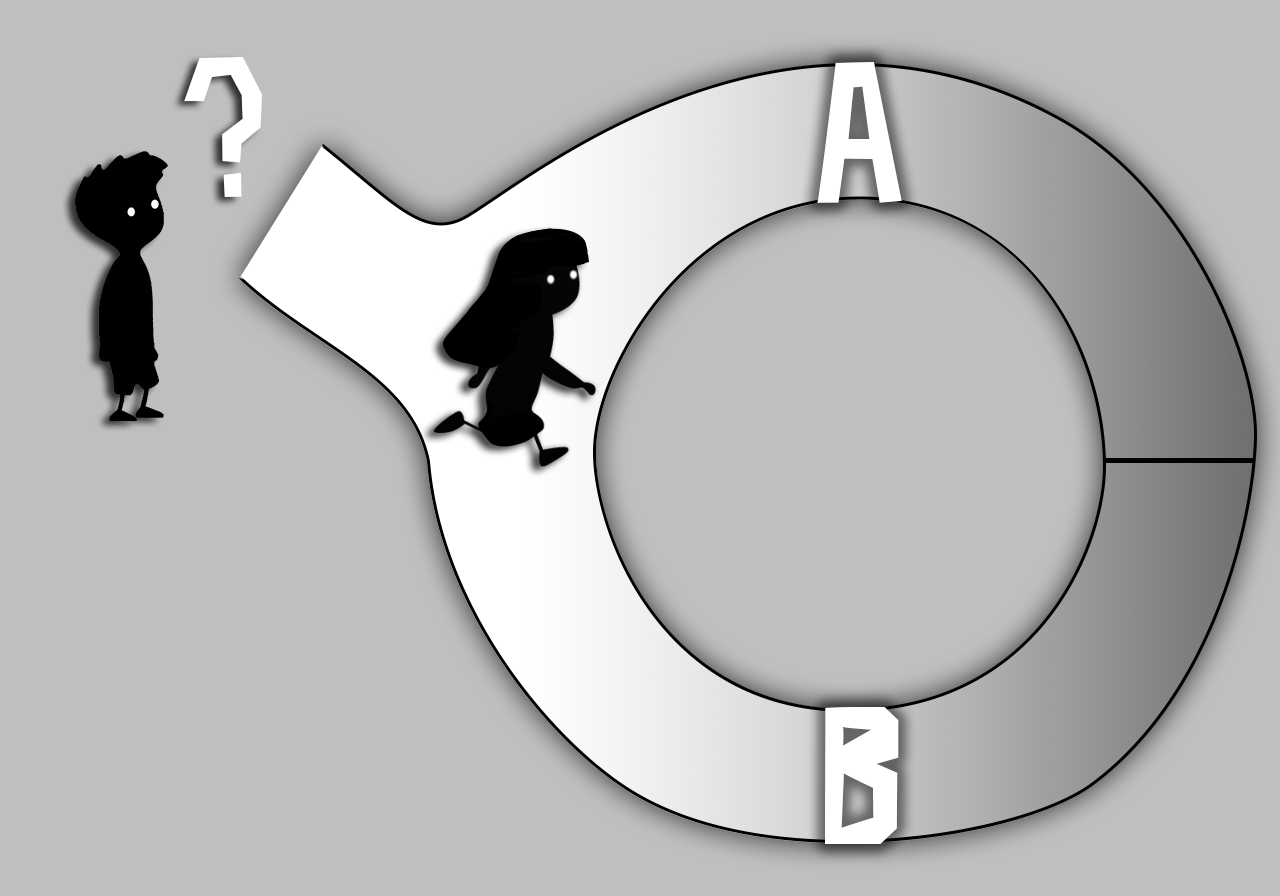
\includegraphics[width=\linewidth]{gfx/graficoJL_ZKP_1}
	\caption*{The cave \citep{ZKPcave:fig}. Peggy takes randomly A or B. Victor awaits outside.}\label{fig:1}
	\endminipage\hfill
	\minipage{0.3\textwidth}
	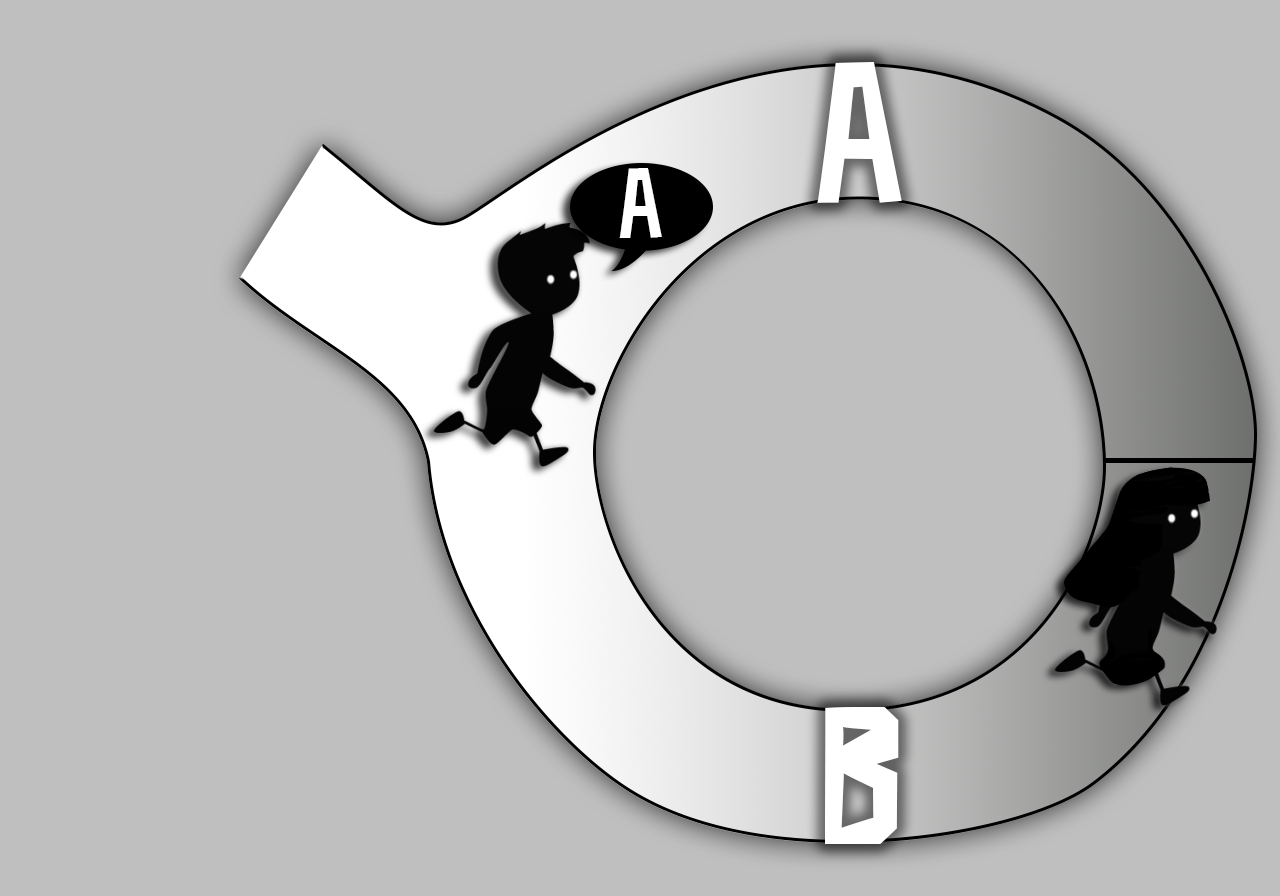
\includegraphics[width=\linewidth]{gfx/graficoJL_ZKP_2}
	\caption*{Victor chooses randomly the returning path for Peggy.}\label{fig:2}
	\endminipage\hfill
	\minipage{0.3\textwidth}%
	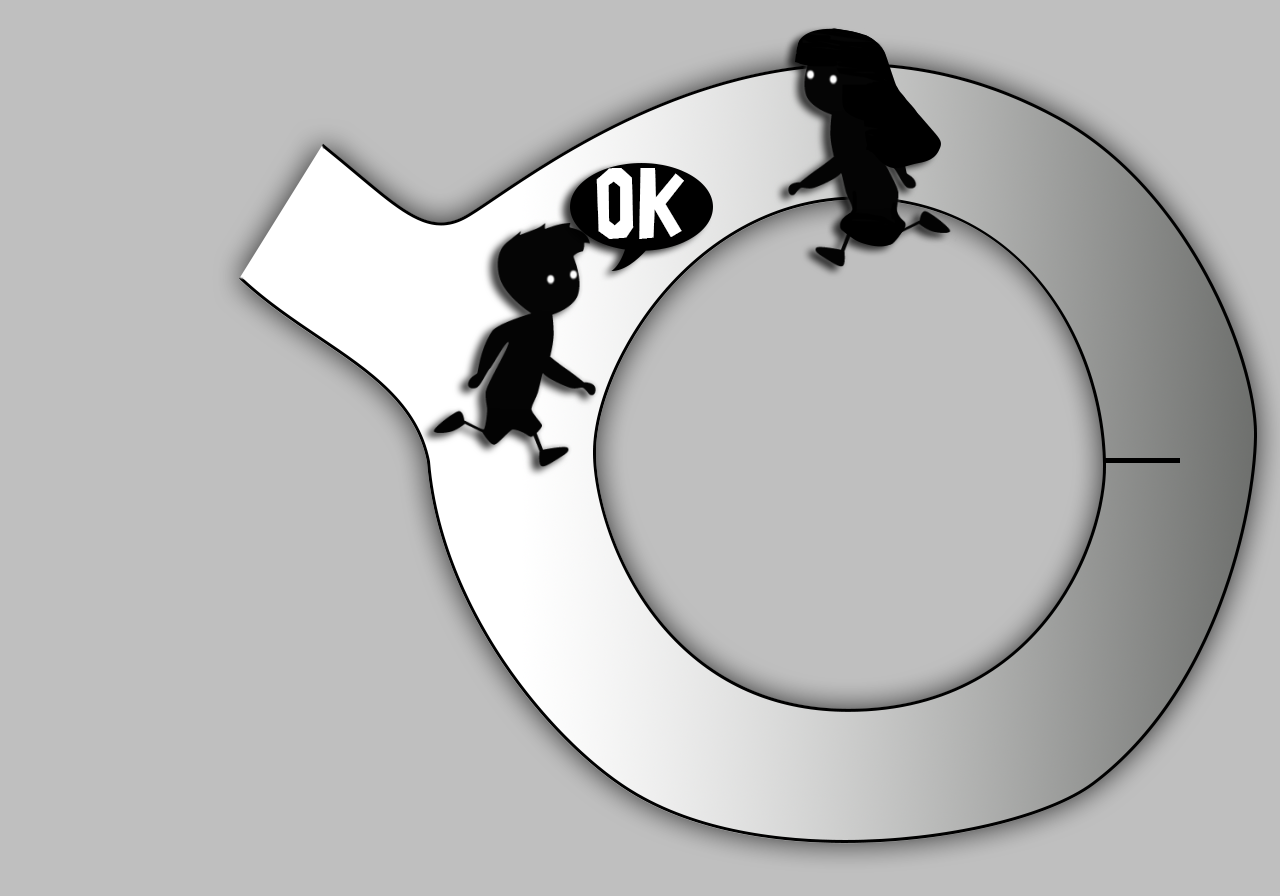
\includegraphics[width=\linewidth]{gfx/graficoJL_ZKP_3}
	\caption*{Peggy returns by the requested path.\\ }\label{fig:3}
	\endminipage
\end{figure}



Many different types of problems are used in the formal study of Zero-Knowledge Proofs, in which those related to number theory and graph theory stand out the most. Theses problems are hard to solve for those who don't know any extra information about the problem, in our story the problem would be opening the door without knowing the magic word. 

The most representative problems in Zero-Knowledge Proofs are the discrete logarithm, the square root modulo a composite integer, the graph isomorphism, finding hamiltonian cycles and the 3-colorability of graphs.

The discrete logarithm consists on, given a cyclic group of prime order, a generator $g$ and an element $y$ in that group, finding the power $s$ such that $g^s=y$, that is, the discrete logarithm base $g$ of $y$, $log_g y$.

The problem of the modular square root involves the quadratic residues theory, which shows us that if the modulus is a prime number, it is easy to find the square root, if it exists, of a given value, but if the modulus is composite, and we don't know its factorization in prime factors, it is hard to even tell if a given value is a quadratic residue, that is, it has square roots.

The graph isomorphism problem consists on given two distinct graphs, tell if there exists an isomorphism between them. This problem has many particular cases easy to solve, but the best known algorithm to solve any instance of the problem is only quasi-polynomial in time, and it is still under revision.

A hamiltonian graph is that with a cycle with every node in the graph, without repetitions.

The 3-colorability of a graph consists on giving each pair of connected nodes two different colors, in a way all the nodes in the graph have only one color, and we used exactly 3 colors.

The hamiltonian cycle and 3-colorability problems have in common that both are categorized in the class of problems known as \textbf{NP}-complete. This means that solving one \textbf{NP}-complete problem is equivalent to solve any other, but to this day no efficient algorithm for any of them is known.


We divide this paper in three parts, during the first one we will study all these problems, starting with defining what we understand a \textit{hard} problem actually is, from a computational point of view, then we will formally describe the mentioned problems, as well as the algorithms that, knowing some extra information (the secret), allow us to solve them.

The second part of this memory will focus on the Zero-Knowledge Proofs themselves, defining what properties must have a proof of this kind, and we will state various proofs related to the problems previously described, proving that each one of them satisfy the definition.

We will first define what an interactive proof formally is, so we then can build on top of it the definition of a Zero-Knowledge Proof, which intuitively is interactive. The first kind of Zero-Knowledge Proof is known as perfect, because no machine would be capable of obtaining any extra information from them. Because this particular definition is very constraining, we will relax it in two ways, the first one, by supposing that our verifier is not malicious, that is, while we interact with it, the verifier won't try to extract extra information from us. The last type of Zero-Knowledge Proofs will be those called computational, in which instead of considering a perfect security against any machine, we consider real world machines, limited in time and memory, and in practice it will give us as much security as the perfect Zero-Knowledge Proofs.


The third part will be dedicated to the practical applications of Zero-Knowledge Proofs. The use of these protocols will let us solve problems related to privacy during communications, increasing application's security and functionality.

One of the most important results in this chapter is the non-interactivity of Zero-Knowledge Proofs, through the Fiat-Shamir heuristic, which uses hash functions, hard to predict in the practice.

Combining many techniques of the Zero-Knowledge Proofs, IBM developed a security suite protocol for privacy preserving, called Identity Mixer. The issuance of credentials uses the Camenisch-Lysyanskaya signature, which most strong features are that it can be performed between two parties, and it can be randomized, in a way some values of the signature change affected by a random parameter, but the signature is still valid.

Then, a certificate can be partially disclosed, that is, when a user presents its certificate to a verifier, only part of the certificate is shown, and the other part is committed with a Zero-Knowledge Proof assuring the hidden values are signed by a valid Camenisch-Lysyanskaya signature, which is also randomized to avoid correlations between different uses of the certificate.

%Identity Mixer accomplishes authentication in a real privacy preserving fashion, removing the need of storing delicate information in the server side, avoiding possible security attacks where the user could not say anything about the security measures to apply. \textit{``If your personal data is never collected, it can not be stolen''} -- Maria Dubovitskaya, from the Identity Mixer team.


Finally, we include an appendix to show some implementations of these algorithms using \texttt{sage}, a Python based mathematical software of free distribution. It offers tools for modular arithmetic so we can focus on the implementation of the protocols instead of writing efficient implementations of modular arithmetic operations to work in other programming languages. These implementations are not related to the Computer Science thesis, which uses the C programming language and focuses on other kind of devices.






\end{otherlanguage}

\endgroup			

\vfill